\documentclass[12pt,a4paper]{article}

% --- Настройка языка и шрифтов для LuaLaTeX ---
\usepackage{fontspec}
\defaultfontfeatures{Ligatures=TeX,Scale=MatchLowercase}

\setmainfont{Alice-Regular}[
    Path=font/,
    Extension=.ttf,
    BoldFont = Alice-Regular,
    ItalicFont = Alice-Regular,
    BoldItalicFont = Alice-Regular,
    BoldFeatures = {FakeBold=1.6},
    ItalicFeatures = {FakeSlant=0.2},
    BoldItalicFeatures = {FakeBold=1.6,FakeSlant=0.2}
]

\newfontfamily\cyrillicfont{Alice-Regular}[
    Path=font/,
    Extension=.ttf,
    BoldFont = Alice-Regular,
    ItalicFont = Alice-Regular,
    BoldItalicFont = Alice-Regular,
    BoldFeatures = {FakeBold=1.6},
    ItalicFeatures = {FakeSlant=0.2},
    BoldItalicFeatures = {FakeBold=1.6,FakeSlant=0.2}
]

\usepackage{polyglossia}
\setmainlanguage{russian}
\setsansfont{TeX Gyre Heros}
\setmonofont{TeX Gyre Cursor}

\usepackage{graphicx}        					          % Графика
\usepackage[protrusion=false]{microtype}       	% Микротипографика
\usepackage{amsmath, amsfonts, amssymb, amsthm}	% Математика
\usepackage{braket} 							              % Braket нотация для квантовой механики
\usepackage{unicode-math} 						          % Современный пакет для математики в LuaLaTeX
\usepackage{longtable}       					          % Таблицы с разрывом страниц
\usepackage{tikz}           					% Рисование
\usepackage[europeanresistors]{circuitikz}		% Рисование электрических схем в европейском стиле
\usepackage{listings}							% Для отображения кода
\usepackage{tabularx}       					% Для таблиц во всю ширину
\usepackage{array}		  						% Для расширенных возможностей таблиц
\usepackage{float}          					% Для точного позиционирования фигур
\usepackage{pgfplots}                           % Для построения графиков
\usepackage{caption}                            % Для настройки подписей к рисункам и таблицам
\usepackage{xfp}                                % Для вычислений в LaTeX
\pgfplotsset{compat=1.18}
\usepackage[a4paper,left=20mm,right=20mm,top=20mm,bottom=20mm]{geometry}

\usetikzlibrary{arrows.meta, positioning, patterns}

% --- Колонтитулы ---
\usepackage{fancyhdr}
\pagestyle{fancy}
\fancyhf{}

\renewcommand{\headrulewidth}{0.4pt}
\renewcommand{\footrulewidth}{0.4pt}
\renewcommand\lstlistingname{Исходный код}

\lstdefinestyle{main}{
	backgroundcolor=\color{gray!8},   
	commentstyle=\color{green!50!black},
	keywordstyle=\color{blue!80!black},
	numberstyle=\small\color{darkgray},
	stringstyle=\rmfamily\color{orange!90!black},
	basicstyle=\ttfamily\small,
	breakatwhitespace=false,         
	breaklines=true,                   
	keepspaces=true,                 
	numbers=left,                    
	numbersep=8pt,                  
	showspaces=false,                
	showstringspaces=false,
	showtabs=false,                  
	tabsize=4
}	

\lstset{style=main}

\newcolumntype{C}{>{\centering\arraybackslash}X}
\renewcommand{\arraystretch}{1.25}

% =========================================================
%         СЛУЖЕБНЫЕ КОМАНДЫ ДЛЯ ВЫЧИСЛЕНИЙ
% =========================================================
\newcommand{\CalcZero} [1]{\fpeval{round((#1),0)}}
\newcommand{\CalcOne}  [1]{\fpeval{round((#1),1)}}
\newcommand{\CalcTwo}  [1]{\fpeval{round((#1),2)}}
\newcommand{\CalcThree}[1]{\fpeval{round((#1),3)}}
\newcommand{\CalcFour} [1]{\fpeval{round((#1),4)}}
\newcommand{\CalcFive} [1]{\fpeval{round((#1),5)}}

% ---------------------------------------------------------
% ОБЩИЕ ДАННЫЕ
% ---------------------------------------------------------
\def\Discipline{Экономика}				           % Название дисциплины
\def\LabTitle{Исследование позиций Vulkan API на рынке вычислительных систем}	 % Название лабораторной работы

\title{
	МИНОБРНАУКИ РОССИИ

	федеральное государственное автономное образовательное учреждение

	высшего образования

	«Национальный исследовательский университет
	«Московский институт электронной техники»
	\vspace{2em}
}
\author{
}
\date{}

\begin{document}

\maketitle
\thispagestyle{fancy}

\begin{center}
\Large Отчёт по дисциплине «\Discipline»\\
«\LabTitle»
\end{center}

\cfoot{Москва 2026}

\pagebreak

\fancyhead[L]{Аннотация} 
\fancyhead[R]{\Discipline}
\fancyfoot[C]{\thepage}

\begin{abstract}
	В последнее время на рынке систем графических API наибольшее распространение получил 
	новичёк в данной индустрии — Vulkan от группы компаний Khronos Group, который 
	представляет из себя эволюцию идей стоящих за OpenGL на базе концепции Mantle от AMD. В этой
	работе будет проанализирована экономическая обоснованность миссии Vulkan, и какая 
	коллизия существует между ним и DirectX12.
\end{abstract}

\section{Что такое графические API?}

Графические API (Application Programming Interface) — это программная обёртка над 
графическим драйвером, которая обрабатывает команды от приложения, переводит их в команды 
отрисовки и передаёт их драйверу видеокарты. Без API необходимо знать спецификацию
каждой модели GPU и переписывать код под каждую отдельную графическую систему. При таких вводных 
единственным валидным решением было максимально избегать графики для приложений на пк, 
как это происходило в случае с DOS, либо создать отдельно техническое решение или найти 
подходящее под задачу уже популярное, под которое будет написан код, что например применялось в 
игровой индустрии — игры писались под конкретную приставку, обязательно учитывая её 
архитектуру.

API стали выоходом из сложившейся ситуации. Они создали 
экономические условия для коммерческого графического 
ПО в секторе индивидульного предпринимательства и 
малого бизнеса, причём как в плане распротранения, так и в плане разработки, так как 
более не было необходимости в том, чтобы под конкретное ПО иметь конкретную аппаратную 
реализацию. Но частные
API не решали коллизии между платформами, а наоборот,
разделяли рынок на фрагменты, которые принадлежали
отдельным компаниям, поддерживающим свои API, только
под свои платформы.

\section{Зарождение первых API и естественная конкуренция на уровне программного 
обеспечения для драйверов графических систем}

Такое затруднительное положение не могло сохраняться долгое время в ситуации, когда
вычислительные мощности продолжают стабильно расти согласно закону Мура\footnote{Закон Мура 
утверждает, что производительность компьютеров удваивается каждые 18-24 месяца, 
выявлен из имперических наблюдений.}, так в 1992 
возник консорциум OpenGL ARB, который ввёл стандарт OpenGL под началом её первого
члена, компании Silicon Graphics\footnote{Впоследствии компания обанкротилась, а её 
штаб-квартира была выкуплена компанией Alphabet и получила название Googleplex.}. 

Новое API было нацелено на создание абстракции обращений к железу для любого языка 
программирования, драйвер сам определяет, как обработать единую абстракцию под конткретного
GPU, к которому обращается приложение, также перед OpenGL ставилась задача создания 
единого стандарта для всех операционных систем. Данное решение было стратигическим. 
Такая гибкость обеспечила консорциуму влиятельных игроков на рынке, чьи продукты они 
фактически обязались обслуживать, согласно их стратегии. Но не все были готовы делигировать
такое одной компании, ведь была такая компания, которая захватила абсолютное большинство 
операционных систем, имя которой Microsoft. 

В 1995 Microsoft запустила своё конкурентное API дающее максимальный функционал для 
Windows систем DirectX, который позиционировался, как инструмент для написания игр под
Windows и впоследствии XBOX. Несмотря на узкую специализацию как факт он стал главным 
идиалогическим конкурентом OpenGL на всё время её существования.

В то время как OpenGL был нейтральным игроком, который пытался вывести индустрию на 
уровень конкуренции не в реализации API, а в конкуренцию реализации одного стандарта, 
DirectX был инструментом влияния Microsoft на рынок, который давал им контроль над 
другими компаниями, ведь если бы OpenGL был единственным API, то у Microsoft не было бы
технической возможности ограничить его использование только для Windows систем, что лишило
бы их аппарата, с помощью которого они могли бы ограничить поддержку ПО или железа других
компаний на основном рынке ПО.\footnote{И это не гипотетический сценарий, далее такой ход 
соверщит Apple, что явно ограничит совместимость стороннего ПО и железа с их платформой}

\section{Роль Khronos Group в истории стандартизации API}

В 2006 году OpenGL ARB на голосовании 3Dlabs, Apple, ATI, Dell, IBM, Intel, Nvidia, SGI и 
Sun Microsystems и множество других более мелких участников проголосовали за передачу 
управления спецификацией OpenGL в Khronos Group, целью ставилось объединение команд
поддерживающих настольные и мобильные с мультимедийными системами.

Но кто же такой Khronos Group? Это некоммерческий отраслевой консорциум, выпускающий 
royalty-free стандарты API, основанный как ответ на продолжающуюся фрагментацию 
стандартов, которая по мнению компаний основателей 3Dlabs, ATI, Evans \& Sutherland, IBM, 
Intel, NVIDIA, SGI и Sun ограничивала развитие индустрии.

Деятельность Khronos Group это поддержка кросплатформенных решений и их обслуживание,
основной статьёй прибыли являются членские взносы управляющих компаний, которые являются
IT гигантами и ведущими игроками сфер компьютерного железа, операционных систем,
разработки игр и программ компьютерной графики.

Khronos Group стала необходима потому, что рынок графики не мог эффективно развиваться 
при полной власти одного производителя. Если бы стандарт контролировался
только Microsoft, он был бы естественно привязан к Windows. Если бы стандарт контролировался 
только AMD, NVIDIA или Intel, остальные производители воспринимали бы
его как инструмент конкурента. Если бы каждая компания создавала собственный API,
разработчики платили бы за это ростом стоимости портирования и тестирования. Таким образом, 
экономический смысл Khronos состоит в снижении транзакционных издержек. 
Блягодаря этому Khronos Group стала нейтрольной прокси-структурой, она заключила в себе идеи 
OpenGL ARB и усилила структуру, в которой компании бы ограничено конкурировали в реализации 
одного стандарта, в рамках формальной структуры. Такая структура лишила Khronos Group 
амбиций, но обеспечила ей экономический успех. 

\section{Кризис контроля над драйвером, эволюция рынка API}

%OpenGL -> Vulkan

%DirectX11 -> DirectX12

В зависимости от полноты команд, драйвера
выполняют разный объём работы, в случае API с высокой степенью абстракции, драйвер
сам решает, как управлять памятью и выполнять синхронизацию

\begin{lstlisting}[language=C++, title={\textbf{Пример инициализации рендера для OpenGL}}]
glUseProgram(program);
glBindBuffer(GL_ARRAY_BUFFER, vbo);
glBindTexture(GL_TEXTURE_2D, texture);
glDrawArrays(GL_TRIANGLES, 0, 3);
\end{lstlisting}
OpenGL-драйвер должен сам понять
\begin{itemize}
	\item какое состояние изменилось
	\item какие объекты активны
	\item валидна ли комбинация состояний
	\item нужно ли перекомпилировать внутренний shader variant
	\item когда реально отправлять команды GPU
	\item как синхронизировать ресурсы
	\item как скрыть задержки
\end{itemize}

В таком подходе удобно то, что программисту не нужно самому строить pipeline\footnote{
Pipeline — графический конвейер, то есть последовательность стадий обработки данных: входные 
вершины, вершинные шейдеры, растеризация, фрагментные шейдеры, тест глубины, смешивание и запись
результата в буфер кадра.
}, 
настраивать синхронизацию как между объектами рендера для видеокарты, так и между
обработкой их функционала в процессоре, но это накладывает ограничения. Такой подход
плохо подходит для эффективной многопоточной генерации команд: GPU является массово
параллельным устройством, а CPU-сторона рендера часто вынуждена последовательно
менять глобальное состояние графического контекста.

Это было применимо во времена, когда рост вычислительных мощностей в основном
достигался за счёт увеличения производительности одного ядра. Когда актуальным стал
подход наращивания количества ядер, как основной вариант увеличения вычислительных
мощностей, драйверно-управляемая модель стала узким местом.

Контроля стало критически не хватать. Отсутствие явной синхронизации, как и отсутствие
явно заданного pipeline, оставляет возможность не столько неправильного результата, 
сколько непредсказуемого времени выполнения и зависимости от эвристик драйвера.
Для программ, которые борются за стабильную задержку кадра и предсказуемую
загрузку CPU, это уже не техническая мелочь, а экономическая проблема: производительность 
железа есть, но полностью извлечь её через старый API трудно.

C другой стороны писать все команды для драйвера самому никому не нужно, это 
бессмысленное действие с экономической точки зрения, такой проект никогда не получиться
окупить. Так как прирост эффективности будет значительный, но количество ошибок в коде, 
категория программиста, их количество, и затраченное время будет кратно отличаться от 
подхода с использованием высоко-абстрактных API не в лучшую сторону.

Встала необходимости о появлении решения, которое будет поддерживать микроконтроль рендера,
в то же время будет абстрагировать машинные команды драйвера, параметры которых
будут управляться из кода, а не подбираться драйвером, который будет принимать не
эффективные решения, а в первую очередь проверенные совместимые\footnote{
Справедливо упомянуть, что драйвер и не может понять, какое решение будет наиболее эффективным, 
потому что не способен узнать контекст, его задача сделать так, чтобы были переданы видеокарте 
команды, которые она будет способна исполнить.
}.

Так AMD в сотрудничестве с DICE начали разработку стандарта Mantle в 2013 году, он 
решал проблему бутылочного горлышка в виде процессора, позволяя синхронизировать нативно
синхронизировать работу по-крайней мере 8 потоков исполнения, позволяло не менять 
состояния рендера, а составить свой pipeline, в который приложение будет само 
отправлять команды, технология была использована DICE в Battlefield 4, что закрепило её
успех, но ограниченная легитимность технологии на рынке из-за её конатации как инструмента 
влияния компании IT гиганта AMD вынудили её передать технологию уже готовую для реализации
на видеокартах от AMD в руки Khronos Group для её развития как нейтральной межвендорной
технологии под новым названием Vulkan. Такое решение было стратегическим ходом против 
монополизации стандартизации компанией Microsoft, с её новым API вдохновлённым Mantle, 
которое являлось продолжателем уже укоренившегося на рынке их старого решения DirectX12.
AMD не могло позволить Microsoft ограничиться одним некросплатформенным API для Windows
систем, чья доминация на рынке операционных систем неоспарима.

\vspace{1em}

\noindent Подход Vulkan заставляет приложение заранее и явно описывать
\begin{itemize}
	\item \texttt{pipeline}
	\item \texttt{layout} ресурсов
	\item \texttt{descriptor sets}
	\item \texttt{barriers}
	\item \texttt{synchronization}
	\item \texttt{memory allocation}
	\item \texttt{command buffers}
	\item \texttt{queues}
\end{itemize}

\begin{lstlisting}[language=C++, title={\textbf{Пример инициализации рендера для Vulkan}}]
vkCreateBuffer / vkAllocateMemory
vkCreateShaderModule
vkCreatePipeline
vkAllocateCommandBuffers
vkBeginCommandBuffer
    vkCmdBindPipeline
    vkCmdBindDescriptorSets
    vkCmdDraw / vkCmdDrawIndexed
vkEndCommandBuffer
vkQueueSubmit
\end{lstlisting}

Приложение отправляет работу в очередь \texttt{VkQueue}, обычно в форме \texttt{VkCommandBuffer}.
Команды, отправленные в одну очередь, стартуют в порядке отправки, но разные очереди
не упорядочены относительно друг друга без явной синхронизации через семафоры, fence
и барьеры памяти.

\begin{center}
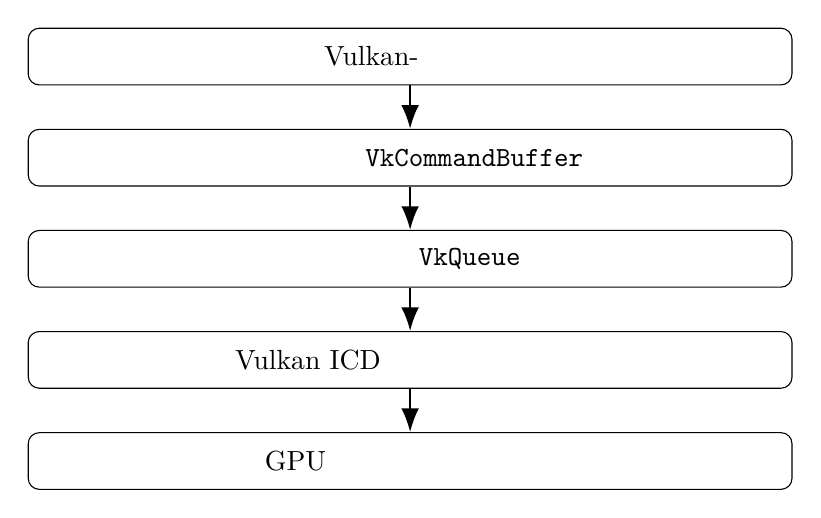
\begin{tikzpicture}[
	node distance=0.55cm,
	box/.style={draw, rounded corners, align=center, minimum width=9.7cm, minimum height=0.72cm},
	arrow/.style={-{Latex[length=3mm]}, thick}
]
\node[box] (app) {Vulkan-приложение};
\node[box, below=of app] (cmd) {Запись команд в \texttt{VkCommandBuffer}};
\node[box, below=of cmd] (queue) {Отправка через \texttt{VkQueue}};
\node[box, below=of queue] (driver) {Vulkan ICD конкретного производителя};
\node[box, below=of driver] (gpu) {GPU исполняет аппаратные команды};

\draw[arrow] (app) -- (cmd);
\draw[arrow] (cmd) -- (queue);
\draw[arrow] (queue) -- (driver);
\draw[arrow] (driver) -- (gpu);
\end{tikzpicture}
\end{center}

Обслуживание и развитие жизнено-необходимого для деятильности многих огромных корпораций 
стандарта дал Khronos Group исключительные позиции на рынке, она стала прокси, 
распространяющим влияние корпораций, издающих своё GPU и выпускающих графическое ПО под 
них, обоюдо выигрышная ситуация, которая ограничивала влияние Microsoft.

Также другие члены консорциума могут принимать прямое участие в развитии стандарта, например
такой член как LunarG, который решает одну из главных экономических проблем, по которым
Vulkan проигрывает более абстрактным API, вроде OpenGL --- необходимость в высококвалифицированных
кадрах, которые будут код писать, отлаживать и поддерживать. LunarG на деньги другого участника
Khronos Group, Valve, занимается разработкой и поддержкой Vulkan SDK, который включает в себя
инструменты для отладки, профилирования и оптимизации приложений на Vulkan, что значительно
снижает необходимую квалификацию для разработки на Vulkan, а значит и общую стоимость проекта
на Vulkan. Так разные компании в рамках одной некоммерческой организации способны работать над
общим стандартом, который впоследствии будет открыто распространяться, несмотря на то, что 
он был оплачен только одним участником.

\section{Успешная консолидация вокруг открытого стандарта}

Победа Khronos Group состояла не в том, что DirectX 12 был вытеснен с Windows, а в
том, что Microsoft не смогла замкнуть всю современную низкоуровневую графику на своей
платформе. Его появление было вызвано техническим кризисом
старых API, в которых слишком большая часть работы перекладывалась на драйвер, и
политико-экономическим риском закрепления современных низкоуровневых API внутри
закрытых платформ Microsoft и Apple. Vulkan стал открытым стандартом, который не отменил 
локальные API, но заставил их
сосуществовать с нейтральной альтернативой, перед которой они выглядели экономическим 
тупиком для сторонних членов индустрии.

Консолидация вокруг Vulkan оказалась выгодной сразу нескольким группам участников.
Для производителей GPU Vulkan снижает риск зависимости от Microsoft или Apple.
AMD, NVIDIA, Intel, Qualcomm, ARM и другие компании могут реализовать один открытый
стандарт, сохраняя конкуренцию на уровне драйвера и железа.
Для разработчиков движков Vulkan даёт общий backend для разных платформ. 
Для Google и Android Vulkan стал способом заменить устаревающий OpenGL ES совре-
менным low-level API. Для Valve и SteamOS Vulkan стал способом строить игровую платфор-
му вне полной зависимости от DirectX. Для Apple Vulkan не стал нативным API, но через
MoltenVK оказался способом доставить Vulkan-приложения поверх Metal.

% Данные: ProPublica Nonprofit Explorer, The Khronos Group Inc, EIN 82-0561169
% Единицы на графиках: млн долларов США

\begin{figure}[H]
\centering
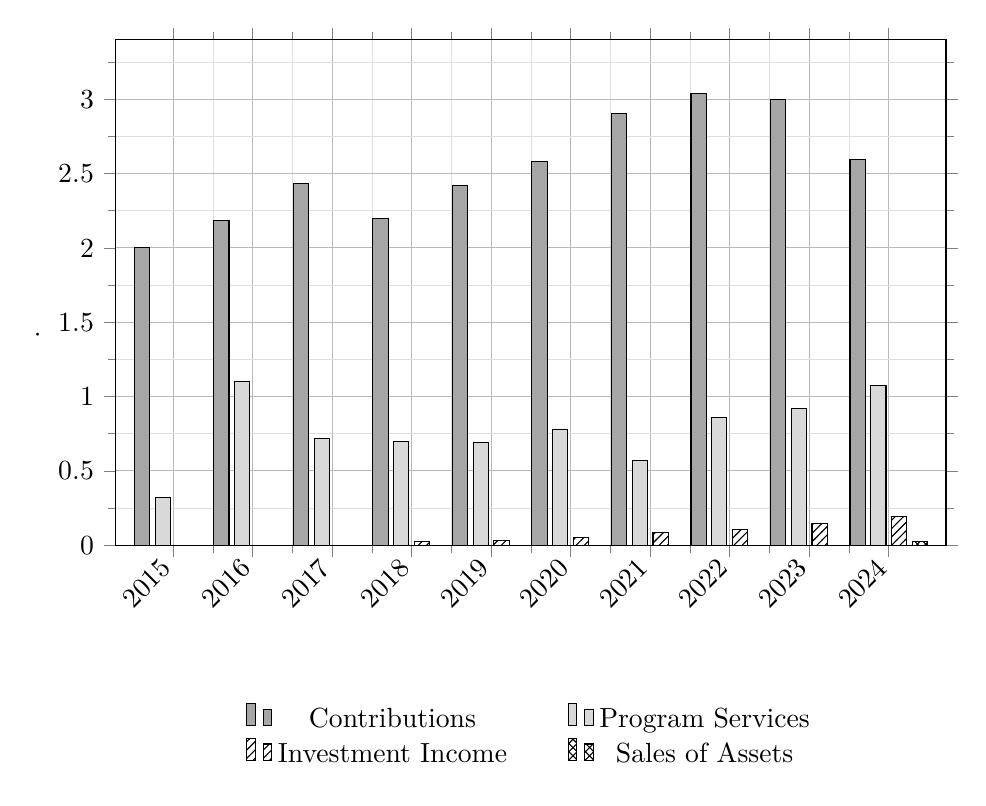
\begin{tikzpicture}
\begin{axis}[
    width=\textwidth,
    height=8cm,
    ybar,
    bar width=5.5pt,
    ymin=0,
    ymax=3.4,
    symbolic x coords={2015,2016,2017,2018,2019,2020,2021,2022,2023,2024},
    xtick=data,
    xticklabel style={rotate=45, anchor=east},
    ylabel={млн. долларов США},
    xlabel={Год},
    grid=both,
    major grid style={line width=0.35pt, draw=gray!55},
    minor grid style={line width=0.15pt, draw=gray!25},
    minor tick num=1,
    tick align=outside,
    enlarge x limits=0.08,
    scaled y ticks=false,
    yticklabel={\pgfmathprintnumber[fixed, precision=1]{\tick}},
    legend style={
        at={(0.5,-0.3)},
        anchor=north,
        legend columns=2,
        draw=none,
        /tikz/every even column/.append style={column sep=0.7cm}
    },
]

% Contributions
\addplot+[
    fill=gray!70,
    draw=black
] coordinates {
    (2015,2.004405)
    (2016,2.185989)
    (2017,2.430157)
    (2018,2.200150)
    (2019,2.417662)
    (2020,2.579151)
    (2021,2.904586)
    (2022,3.037850)
    (2023,2.999539)
    (2024,2.592490)
};

% Program Services
\addplot+[
    fill=gray!30,
    draw=black
] coordinates {
    (2015,0.319409)
    (2016,1.099221)
    (2017,0.718736)
    (2018,0.694880)
    (2019,0.692980)
    (2020,0.779064)
    (2021,0.568947)
    (2022,0.859208)
    (2023,0.918811)
    (2024,1.071041)
};

% Investment Income
\addplot+[
    fill=white,
    pattern=north east lines,
    pattern color=black,
    draw=black
] coordinates {
    (2015,0.000047)
    (2016,0.000174)
    (2017,0.000456)
    (2018,0.024058)
    (2019,0.032491)
    (2020,0.049114)
    (2021,0.086344)
    (2022,0.105622)
    (2023,0.142710)
    (2024,0.190931)
};

% Sales of Assets
\addplot+[
    fill=white,
    pattern=crosshatch,
    pattern color=black,
    draw=black
] coordinates {
    (2015,0.000000)
    (2016,0.000000)
    (2017,0.000000)
    (2018,0.000000)
    (2019,0.000000)
    (2020,0.000000)
    (2021,0.000000)
    (2022,0.000000)
    (2023,0.000000)
    (2024,0.026895)
};

\legend{
    Contributions,
    Program Services,
    Investment Income,
    Sales of Assets
}

\end{axis}
\end{tikzpicture}
\end{figure}

% Увеличенный график малых статей дохода
% Единицы: тыс. долларов США

\begin{figure}[H]
\centering
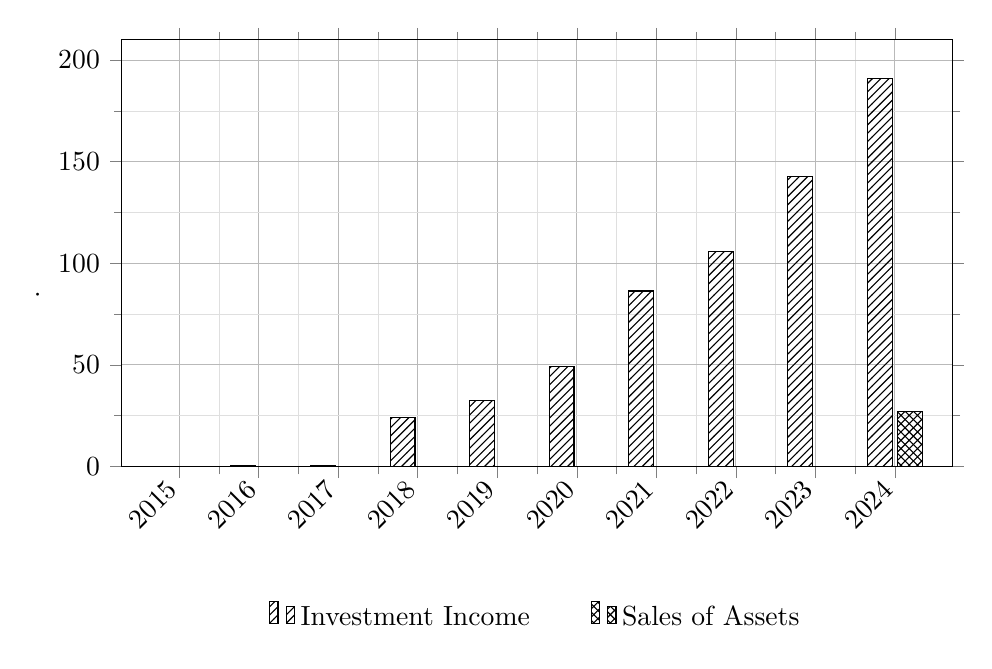
\begin{tikzpicture}
\begin{axis}[
    width=\textwidth,
    height=7cm,
    ybar,
    bar width=9pt,
    ymin=0,
    ymax=210,
    symbolic x coords={2015,2016,2017,2018,2019,2020,2021,2022,2023,2024},
    xtick=data,
    xticklabel style={rotate=45, anchor=east},
    ylabel={тыс. долларов США},
    xlabel={Год},
    grid=both,
    major grid style={line width=0.35pt, draw=gray!55},
    minor grid style={line width=0.15pt, draw=gray!25},
    minor tick num=1,
    tick align=outside,
    enlarge x limits=0.08,
    scaled y ticks=false,
    legend style={
        at={(0.5,-0.3)},
        anchor=north,
        legend columns=2,
        draw=none,
        /tikz/every even column/.append style={column sep=0.7cm}
    },
]

% Investment Income, тыс. долларов
\addplot+[
    fill=gray!55,
	pattern=north east lines,
    draw=black
] coordinates {
    (2015,0.047)
    (2016,0.174)
    (2017,0.456)
    (2018,24.058)
    (2019,32.491)
    (2020,49.114)
    (2021,86.344)
    (2022,105.622)
    (2023,142.710)
    (2024,190.931)
};

% Sales of Assets, тыс. долларов
\addplot+[
    fill=white,
    pattern=crosshatch,
    pattern color=black,
    draw=black
] coordinates {
    (2015,0.000)
    (2016,0.000)
    (2017,0.000)
    (2018,0.000)
    (2019,0.000)
    (2020,0.000)
    (2021,0.000)
    (2022,0.000)
    (2023,0.000)
    (2024,26.895)
};

\legend{
    Investment Income,
    Sales of Assets
}

\end{axis}
\end{tikzpicture}
\end{figure}

% Данные:
% 2004--2010: вручную извлечены из PDF Form 990.
% 2011--2024: ProPublica Nonprofit Explorer, The Khronos Group Inc, EIN 82-0561169.
%
% Единицы: млн долларов США.
%
% Важно:
% 2004--2007: основная выручка отражалась как Membership dues and assessments.
% 2008--2024: членские платежи больше не выводятся отдельной старой строкой line 3
% в той же форме; в агрегированных данных ProPublica они входят в Contributions.
% Поэтому серия Membership dues заполнена только за 2004--2007, чтобы не удваивать данные.

\begin{figure}[H]
\centering
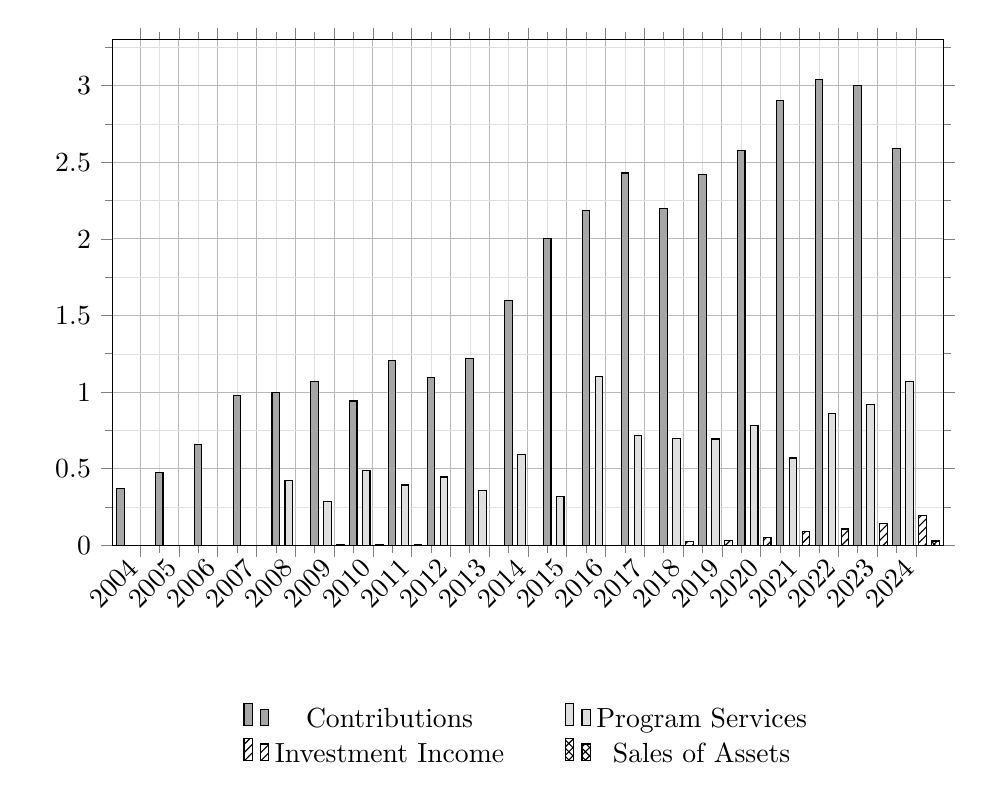
\begin{tikzpicture}
\begin{axis}[
    width=\textwidth,
    height=8cm,
    ybar,
    bar width=2.7pt,
    ymin=0,
    ymax=3.3,
    symbolic x coords={2004,2005,2006,2007,2008,2009,2010,2011,2012,2013,2014,2015,2016,2017,2018,2019,2020,2021,2022,2023,2024},
    xtick=data,
    xticklabel style={rotate=45, anchor=east},
    ylabel={млн долларов США},
    xlabel={Год},
    grid=both,
    major grid style={line width=0.35pt, draw=gray!55},
    minor grid style={line width=0.15pt, draw=gray!25},
    minor tick num=1,
    tick align=outside,
    enlarge x limits=0.035,
    scaled y ticks=false,
    yticklabel={\pgfmathprintnumber[fixed, precision=1]{\tick}},
    legend style={
        at={(0.5,-0.3)},
        anchor=north,
        legend columns=2,
        draw=none,
        /tikz/every even column/.append style={column sep=0.7cm}
    },
]

% Contributions
\addplot+[
    fill=gray!70,
    draw=black
] coordinates {
	(2004,0.367759)
    (2005,0.474476)
    (2006,0.658513)
    (2007,0.977765)
    (2008,0.997210)
    (2009,1.067580)
    (2010,0.941000)
    (2011,1.205888)
    (2012,1.093780)
    (2013,1.216000)
    (2014,1.595000)
    (2015,2.004405)
    (2016,2.185989)
    (2017,2.430157)
    (2018,2.200150)
    (2019,2.417662)
    (2020,2.579151)
    (2021,2.904586)
    (2022,3.037850)
    (2023,2.999539)
    (2024,2.592490)
};

% Program Services
\addplot+[
    fill=gray!25,
    draw=black
] coordinates {
    (2004,0.000000)
    (2005,0.000000)
    (2006,0.000000)
    (2007,0.000000)
    (2008,0.419310)
    (2009,0.286210)
    (2010,0.489477)
    (2011,0.392520)
    (2012,0.444681)
    (2013,0.355572)
    (2014,0.589650)
    (2015,0.319409)
    (2016,1.099221)
    (2017,0.718736)
    (2018,0.694880)
    (2019,0.692980)
    (2020,0.779064)
    (2021,0.568947)
    (2022,0.859208)
    (2023,0.918811)
    (2024,1.071041)
};

% Investment Income
\addplot+[
    fill=white,
    pattern=north east lines,
    pattern color=black,
    draw=black
] coordinates {
    (2004,0.000000)
    (2005,0.000000)
    (2006,0.000000)
    (2007,0.000000)
    (2008,0.000000)
    (2009,0.000811)
    (2010,0.001189)
    (2011,0.000804)
    (2012,0.000289)
    (2013,0.000106)
    (2014,0.000010)
    (2015,0.000047)
    (2016,0.000174)
    (2017,0.000456)
    (2018,0.024058)
    (2019,0.032491)
    (2020,0.049114)
    (2021,0.086344)
    (2022,0.105622)
    (2023,0.142710)
    (2024,0.190931)
};

% Sales of Assets
\addplot+[
    fill=white,
    pattern=crosshatch,
    pattern color=black,
    draw=black
] coordinates {
    (2004,0.000000)
    (2005,0.000000)
    (2006,0.000000)
    (2007,0.000000)
    (2008,0.000000)
    (2009,0.000000)
    (2010,0.000000)
    (2011,0.000000)
    (2012,0.000000)
    (2013,0.000000)
    (2014,0.000000)
    (2015,0.000000)
    (2016,0.000000)
    (2017,0.000000)
    (2018,0.000000)
    (2019,0.000000)
    (2020,0.000000)
    (2021,0.000000)
    (2022,0.000000)
    (2023,0.000000)
    (2024,0.026895)
};

\legend{
    Contributions,
    Program Services,
    Investment Income,
    Sales of Assets
}

\end{axis}
\end{tikzpicture}
\end{figure}

\end{document}